\documentclass[10pt, a4paper, italian]{article}
\usepackage[T1]{fontenc}
\usepackage[utf8]{inputenc}
\usepackage{amsmath, amssymb, amsthm, thmtools, amsfonts, mathtools}
\usepackage{nicefrac}
\usepackage{calc}
\usepackage[pdftex, hyperindex, plainpages=false]{hyperref}
\usepackage[nameinlink]{cleveref} %load before classicthesis (clash)
%\usepackage[nochapters,pdfspacing]{classicthesis}
\usepackage{siunitx}
\usepackage[siunitx]{circuitikz}

\usepackage[a4paper]{geometry}
\usepackage{float}
\usepackage{mdframed}
\usepackage{titling}
\usepackage{booktabs}
\usepackage{graphicx}
\usepackage{caption, subcaption}
\usepackage{xcolor}
\usepackage[italian]{babel}
\usepackage{pgfplots}
\usepackage{listings}
%\usepackage{lmodern}
\usepackage{url}
\usepackage{enumitem}
\usepackage{tikz} %loads after classicthesis (xcolor incompat)

% lets graphicx know path where figures to be included are found
\graphicspath{{../figs/}}
\makeatletter
\def\input@path{{../figs/}}
%or: \def\input@path{{/path/to/folder/}{/path/to/other/folder/}}
\makeatother

% tikz pgf plots setup
\usepgfplotslibrary{external}
\pgfplotsset{compat=1.15}
%\tikzexternalize

% spaces and significant digits/figures for measurements
\sisetup{free-standing-units, space-before-unit, number-unit-product = \;,
scientific-notation = false, round-mode = figures, round-precision = 1,}

% turns all (hyperlinked) references black [default is blue]
\hypersetup{
	linktoc=all,
	colorlinks=true,
	linkcolor=black
}

% code listings config
%\lstset{
%language=Python,
%basicstyle=\ttfamily,
%columns=fullflexible,
%keepspaces=true,
%}

% mdframed (for boxed text) configuration
\mdfsetup{linewidth=0.6pt}

% Default fixed font does not support bold face
\DeclareFixedFont{\ttb}{T1}{txtt}{bx}{n}{12} % for bold
\DeclareFixedFont{\ttm}{T1}{txtt}{m}{n}{12}  % for normal

% Custom colors
\usepackage{color}
\definecolor{deepblue}{rgb}{0,0,0.5}
\definecolor{deepred}{rgb}{0.6,0,0}
\definecolor{deepgreen}{rgb}{0,0.5,0}

% Commands 
\newcommand{\executeiffilenewer}[3]{%
	\ifnum\pdfstrcmp{\pdffilemoddate{#1}}%
		{\pdffilemoddate{#2}}>0%
	{\immediate\write18{#3}}\fi%
}
% input .svg --> .pdf_tex graphs
%\newcommand{\includesvg}[1]{%
%	\executeiffilenewer{#1.svg}{#1.pdf}%
%	{inkscape -z -D --file=#1.svg %
%	--export-pdf=#1.pdf --export-latex}%
%	\input{#1.pdf_tex}%
%}
% Thanks UniPi's Department of Physics E. Fermi
\newcommand{\thanksdf}{(\thanks{Dipartimento di Fisica E.~Fermi,%
Universit\`a di Pisa - Pisa, Italy.}\;)}

% hyperlink to email address
\newcommand{\mail}[1]{\href{mailto:#1}{\textsf{#1}}}

% \vec for bold vectors, instead of overarrows (now "\arrvec")
\let\arrvec=\vec
\renewcommand{\vec}[1]{\boldsymbol #1}
% replaces straight phi with slanted phi
\renewcommand{\phi}{\varphi}
% replaces straight eps with curved epsilon
\newcommand{\eps}{\varepsilon}
% abbreviation for (sub_/super^)scripts of \lim, \sum,... in inline math
\newcommand{\ds}{\displaystyle}

% blackboard/number set letters
\newcommand{\CC}{\mathbb C}
\newcommand{\HH}{\mathbb H}
\newcommand{\KK}{\mathbb K}
\newcommand{\NN}{\mathbb N}
\newcommand{\PP}{\mathbb P}
\newcommand{\QQ}{\mathbb Q}
\newcommand{\RR}{\mathbb R}
\newcommand{\ZZ}{\mathbb Z}

\newcommand{\Abs}[1]{{\left\Vert #1\right\Vert}}
\newcommand{\enclose}[1]{{\left( #1 \right)}}
\newcommand{\Enclose}[1]{{\left[ #1 \right]}}
\newcommand{\floor}[1]{\left\lfloor #1 \right\rfloor}
\newcommand{\ceil}[1]{\left\lceil #1 \right\rceil}
\newcommand{\To}{\rightrightarrows}

% Math operators
\DeclareMathOperator{\divergence}{div}
\renewcommand{\div}{\divergence}
\DeclareMathOperator{\Imaginarypart}{Im}
\renewcommand{\Im}{\Imaginarypart}
\DeclareMathOperator{\Realpart}{Re}
\renewcommand{\Re}{\Realpart}
%\DeclareMathOperator{\arg}{arg}
\DeclareMathOperator{\tg}{tg}
\DeclareMathOperator{\arctg}{arctg}
\DeclareMathOperator{\settsinh}{settsinh}
\DeclareMathOperator{\settcosh}{settcosh}
\DeclareMathOperator{\tr}{tr}
\DeclareMathOperator{\im}{im}
\DeclareMathOperator{\sgn}{sgn}
\DeclareMathOperator{\diag}{diag}

\DeclarePairedDelimiter{\norm}{\lVert}{\rVert}
\DeclarePairedDelimiter{\scalar}{\langle}{\rangle}

% Logarithm with arbitrary base.
% -> log_10
\newcommand{\llog}[1][10]{\log_{#1}}

% Absolute value.
% -> |x|
\newcommand{\abs}[1]{\left| #1 \right|}

% Powers.
% -> x^a
\newcommand{\power}[2][2]{\left( #2 \right)^{#1}}

% Square.
% -> x^2
\newcommand{\sq}[1]{\power[2]{#1}}

% Expansion of the binomial coefficient.
% -> n1!/(n2!(n1 - n2)!)
\newcommand{\binomexpr}[2]{\frac{#1!}{#2!(#1 - #2)!}}

% Expression evaluation at a given point with square brackets.
% -> [x]_{a}
\newcommand{\at}[2]{\left[ #1\right]_{\makebox[-1pt][l]{${\scriptstyle#2}$}}}

% Expression evaluation in an interval.
% -> [x] _{a}^{b}
\newcommand{\eval}[3]{\left.#1%
  \right|_{\makebox[-1pt][l]{${\scriptstyle#2}$}}^{\makebox[-1pt][l]{${\scriptstyle#3}$}}}

% Upright d in math mode (for differentials).
% -> d
\newcommand{\ud}{\mathrm{d}}

% Differential.
% -> dx
\newcommand{\diff}[1][x]{\,\ud{#1}}

% Base command for defining derivatives.
% -> df/dx or d^kf/dx^k
\newcommand{\basederivative}[4][]{%
  \displaystyle%
  \ifx\\#1\\\frac{#4#2}{#4#3}%
  \else%
  \frac{#4^#1#2}{#4#3^#1}%
  \fi%
}

% Total derivative.
% -> df/dx(x) or d^kf/dx^k(x)
\newcommand{\td}[4][]{%
  \basederivative[#1]{#2}{#3}{\ud}%
  \ifx\\#4\\%
  \else%
  \mkern-4mu\left(#4\right)%
  \fi%
}

% Partial derivative.
% -> df/dx(x) or d^kf/dx^k(x)
\newcommand{\pd}[4][]{%
  \basederivative[#1]{#2}{#3}{\partial}%
  \ifx\\#4\\%
  \else%
  \mkern-4mu\left(#4\right)%
  \fi%
}

\newcommand{\intinf}{\int_{-\infty}^{\infty}\!\!\!}

\newcommand{\cinterval}[2]{\left[\, #1,~#2 \,\right]}

\newcommand{\linterval}[2]{\left[\, #1,~#2 \,\right)}

\newcommand{\rinterval}[2]{\left(\, #1,~#2 \,\right]}

\newcommand{\ointerval}[2]{\left(\, #1,~#2 \,\right)}

\newcommand{\prob}[1]{\displaystyle P\left(#1\right)}

\newcommand{\pvalue}{\emph{$p$-value}}

\newcommand{\cond}{\,|\,}

\newcommand{\expect}[1]{\displaystyle E\left[#1\right]}

\newcommand{\mom}[2][]{\displaystyle {\cal M}_{#2}\ifx\\#1\\\else(#1)\fi}

\newcommand{\momalg}[1]{\displaystyle \lambda_{#1}}

\newcommand{\momcen}[1]{\displaystyle \mu_{#1}}

\newcommand{\skewness}{\displaystyle \gamma_1}

\newcommand{\kurtosis}{\displaystyle \gamma_2}

\newcommand{\charf}[1][x]{\phi_{#1}}

\newcommand{\momgenf}[1][x]{M_{#1}}

\newcommand{\fwhm}{{\scriptstyle \textsc{FWHM}}}

\newcommand{\hwhm}{{\scriptstyle \textsc{HWHM}}}

\newcommand{\median}{\mu_{\nicefrac{1}{2}}}

\newcommand{\var}[1]{\ensuremath{\text{Var}\left(#1\right)}}

\newcommand{\cov}[2]{\ensuremath{\text{Cov}\left(#1, #2\right)}}

\newcommand{\corr}[2]{\ensuremath{\text{Corr}\left(#1, #2\right)}}

\newcommand{\like}{\mathcal L}

\newcommand{\likelihood}[2][]{\like\ifx\\#2\\\else(#2\ifx\\#1\\\else;#1\fi)\fi}

\newcommand{\chisq}{\ensuremath{\chi^2}}

\newcommand{\chisquare}[2][]{\chisq\ifx\\#2\\\else(#2\ifx\\#1\\\else;#1\fi)\fi}

\newcommand{\loglikelihood}[2][]{\log\likelihood[#1]{#2}}

\newcommand{\pdf}[3][]{#2(#3\ifx\\#1\\\else;#1\fi)}

\newcommand{\binomialpdf}[2][]{\pdf[#1]{\mathcal B}{#2}}

\newcommand{\multinomialpdf}[2][]{\pdf[#1]{\mathcal M}{#2}}

\newcommand{\poissonpdf}[2][]{\pdf[#1]{\mathcal P}{#2}}

\newcommand{\uniformpdf}[2][]{\pdf[#1]{u}{#2}}

\newcommand{\exponentialpdf}[2][]{\pdf[#1]{\varepsilon}{#2}}

\newcommand{\gausspdf}[2][]{\pdf[#1]{N}{#2}}

\newcommand{\chisquarepdf}[2][]{\pdf[#1]{\wp}{#2}}

\newcommand{\cauchypdf}[2][]{\pdf[#1]{c}{#2}}

\newcommand{\erf}[1]{\ensuremath{\text{erf}\left(#1\right)}}

\newcommand{\dccases}[4][]{#2 \ifx\\#2\\\else=\fi %
  \begin{cases}
    \displaystyle #3 & \text{per variabili discrete}\\
    \displaystyle #4 & \text{per variabili continue}#1
  \end{cases}
}
% sub/super-scriptable for all symbol as math operator 
\newcommand\Scaleforall[1]{\vcenter{\hbox{\scalefont{#1}$\forall$}}}

\DeclareMathOperator*\forevery{%
  \vphantom\sum
  \mathchoice{\Scaleforall{2}}{\Scaleforall{1.4}}{\Scaleforall{1}}{\Scaleforall{0.75}}}
\geometry{left=2cm, right=2cm, top=2cm, bottom=2cm}

% makes all hyperlinks the same color as text
\hypersetup{
	linktoc=all,
	colorlinks=false,
	linkcolor=black
	}
% lets graphicx know path where figures to be included are found
\graphicspath{{../figs/}}

\author{Gruppo 1.AC \\ Matteo Rossi, Bernardo Tomelleri}
\title{Es12: Misura del rapporto $h/e$ per effetto fotoelettrico}
\begin{document}
\date{\today}
\maketitle

%=======================
\section{Scopo dell'esperienza}
Scopo dell'esperienza è verificare l'effetto fotoelettrico e la dipendenza
lineare tra energia e frequenza dei fotoni, dunque da questa ricavare una stima
del rapporto tra la costante di Planck e la carica dell'elettrone $h/e$
utilizzando il metodo del potenziale frenante (implementato per la prima volta
da R.A. Millikan, 1914-16).

\section{Metodo di misura del potenziale frenante}
L'effetto fotoelettrico prevede che un elettrone può essere estratto da un
metallo assorbendo un fotone con energia superiore al lavoro di estrazione
$W_{0}$ e venire emesso con energia cinetica pari a
\begin{equation}\label{eq: cons}
E = h \nu - W_0
\end{equation}
dove $\nu$ è la frequenza della radiazione elettromagnetica incidente sul
metallo e $h \nu$ l'energia trasportata da ogni fotone di cui è costituita.

Nel nostro apparato sperimentale i \emph{fotoelettroni}, i.e. gli elettroni
estratti per effetto fotoelettrico dal catodo di una cella fotoelettrica
Leybold 5587 determinano una \emph{fotocorrente} verso l'anodo, che
colleghiamo all'ingresso di un picoamperometro (mod. Keithley 595: Quasistatic
C-V Meter) per riuscire a misurarne l'intensità $I_{ph}$.

Questi elettroni vengono `frenati' da un campo elettrico di verso concorde al
loro moto, generato da una tensione regolabile $V\ped{bias}$ applicata tra
anodo e catodo, al fine di trovare la differenza di potenziale critica $V_0$
per cui l'intensità di corrente $I_{ph}(V\ped{bias})$ si annulla.
La barriera di potenziale $eV_0$ corrispondente alla tensione che arresta il
flusso di fotoelettroni ci fornisce quindi una stima della massima
energia cinetica da essi raggiunta, che possiamo mettere in relazione alla
frequenza della radiazione incidente (per conservazione dell'energia
\cref{eq: cons})
\begin{equation}\label{eq: V0}
V_0 = \frac{h}{e} \nu - \frac{W_0}{e}
\end{equation}

Questa è proprio la relazione lineare tra energia e frequenza che intendiamo
verificare, tramite cui possiamo stimare il valore del rapporto $h/e$ a
partire dal coefficiente angolare della retta di best-fit.

Assumendo come valori esatti $e = 1.602176634 \times 10^{-19}{\coulomb}$ e
$h = 6.62607015 \times 10^{-34} \; \si{\J\s} $ il valore atteso del loro
rapporto è
\begin{equation}\label{eq: e/h}
\left(\frac{h}{e}\right)\ped{exp} = 4.14 \times 10^{-15} \; \si{\V\s}
\end{equation}

\subsection{Sovrapposizione di correnti spurie}
In realtà il nostro apparato è racchiuso da una scatola metallica per
schermarlo dalla luce e dal rumore elettronico ambientale, ma la misura
di $h/e$ è affetta da diverse fonti di errore sistematico.

La corrente $I(V\ped{bias})$ che misuriamo tra anodo e catodo in realtà è il
risultato di una combinazione con altre correnti ``inverse'' (cioè
associate alla migrazione di elettroni dall'anodo verso il catodo) alla
fotocorrente catodica, che continuano a essere presenti anche per valori
di $V\ped{bias} > V_0$.

Queste ci permettono al più di ricavare una stima preliminare dell'ordine di
grandezza di $V_0$, ricercando la transizione fra il regime in cui
misuriamo $I>0$ o $I \sim 0$ dalle curve corrente-tensione ottenute al variare
della lunghezza d'onda (di cui riportiamo un esempio in \cref{fig: 546nm}).

\begin{figure}[htbp]
    \centering
	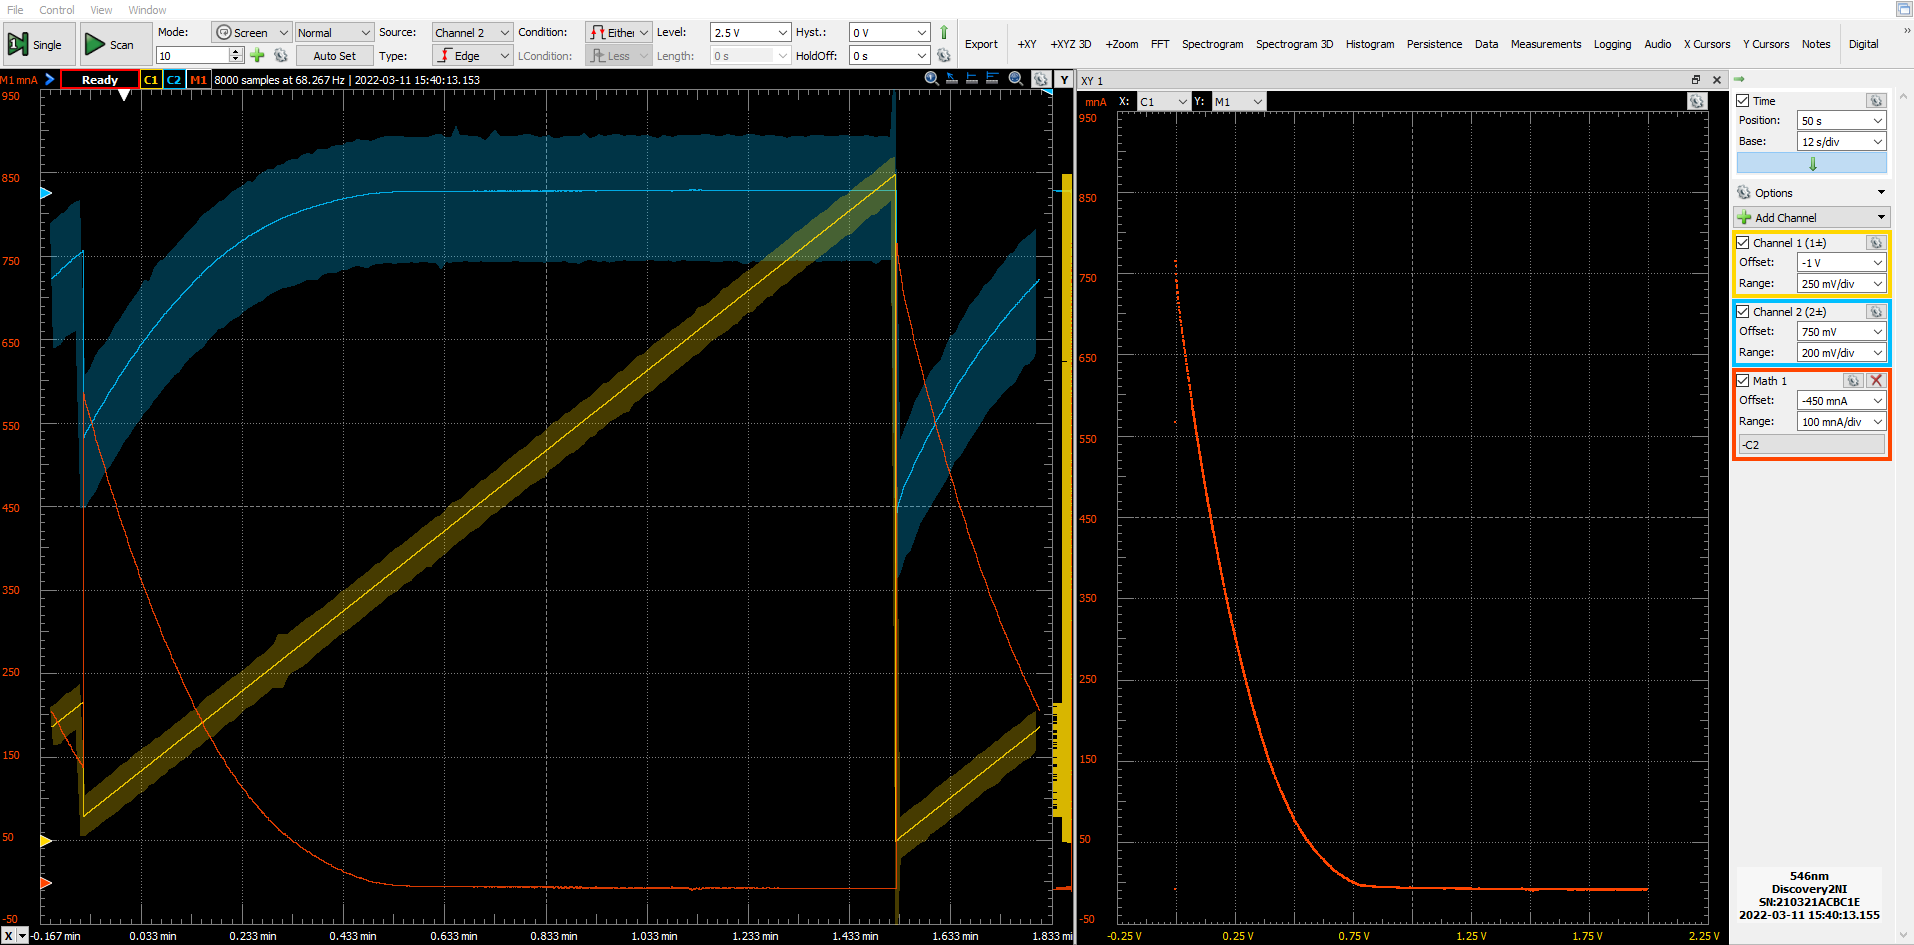
\includegraphics[width=\textwidth]{546nm}
    \caption{Acquisizione della curva tensione $V\ped{bias}(t)$ (CH1)
    corrente (Math1 in mnA = pA) per lunghezza d'onda $546 \; \si{n\m}$, in
    cui si vede un ginocchio verso $I=0$ intorno a
    $V_0 \approx 0.75 \; \si{\V}$
    \label{fig: 546nm}}
\end{figure}

Ipotizziamo che queste correnti siano dovute alla sovrapposizione di vari
effetti di natura diversa:
\begin{enumerate}
        \item emissione di fotoelettroni dall'anodo, dovuta a imperfezioni nel
        sistema di illuminazione del catodo che può investire anche l'anodo
        (schematizzato in \cref{fig: lamp});
        \item estrazione di elettroni dall'anodo per effetto termoionico
        (corrente oscura).
        \item connessione ohmica tra gli elettrodi dovuta al non perfetto
        isolamento delle guaine di rivestimento dei cavi.
    \end{enumerate}

Nonostante ci aspettiamo contributi di gran lunga minoritari rispetto alla
fotocorrente in assenza di bias tra gli elettrodi, già da adesso notiamo come
i primi due crescano con la tensione di frenamento (per questi elettroni il
campo elettrico è accelerante) diventando sempre più significativi,
specialmente per tensioni prossime a quella di azzeramento $V_0$ dove
$I_{ph}$ si estingue.

Per poter ovviare a queste contaminazioni date dalle correnti inverse
$I = I_{ph} + I\ped{inv}$, ne teniamo conto misurandone l'intensità, la quale
supponiamo per semplicità linearmente dipendente dalla tensione di bias
\begin{equation}\label{eq: I0fit}
I\ped{inv} = bV + I_0
\end{equation}

per cui ci aspettiamo che i parametri $b$ e $I_0$ non dipendano dalla
frequenza della luce incidente, ma puramente dalle caratteristiche fisiche
della cella fotoelettrica. Nel caso particolare la corrente inversa fosse di
natura puramente ohmica ci aspettiamo proporzionalità diretta
$I\ped{inv} \propto V\ped{bias}$ e offset $I_0$ nullo.

Assumendo una distribuzione di Fermi-Dirac per gli elettroni liberi nella
banda di conduzione del catodo, senza tenere conto dell'interazione con i
fotoni, possiamo modellare l'andamento della fotocorrente in funzione della
tensione di frenamento come una legge di potenza che si annulla\footnote{
indicando con $\theta(x)$ la funzione gradino di Heaviside $\theta(x) \coloneqq
\begin{cases} 1 & x > 0 \\ 0 & x \leq 0 \end{cases}$} in $V_0$
\[
I_{ph} = (V_0 - V)^{3/2} \theta(V_0 - V)
\]

Dunque possiamo ottenere una misura più attendibile della tensione di
azzeramento -per ogni valore della lunghezza d'onda- tramite fit alla corrente
complessiva, con un modello del tipo:
\begin{equation}\label{eq: Ifit}
I(V) = I_{ph} + I\ped{inv} = a(V_0 - V)^\alpha \theta(V_0 - V) + bV + I_0
\end{equation}

Come prima è ragionevole assumere che l'esponente $\alpha$ sia indipendente
dalle caratteristiche della luce incidente (visto che fisicamente dipende
dalla densità degli stati elettronici del metallo nella banda di conduzione e
da effetti legati all'interazione dei fotoelettroni con il bulbo della
fotocella).

Mentre il parametro $a$, legato alla normalizzazione della fotocorrente,
dovrebbe racchiudere la dipendenza dalla frequenza della luce incidente, poiché
vi dipendono sia l'intensità spettrale della lampada nella banda di selezione
del filtro, che la sezione d'urto dell'effetto fotoelettrico alla
corrispondente energia.

%=======================
\section{Descrizione delle misure}
Nella realizzazione pratica dell'esperimento la radiazione luminosa è
inizialmente emessa secondo uno spettro -praticamente- continuo da una
lampada a LED, viene collimato da un diaframma circolare, dunque focalizzato
da un paio di lenti convergenti prima di essere filtrato e incidere sul catodo
della fotocella (come visto in \cref{fig: lamp}).
\begin{figure}[htbp]
    \centering
	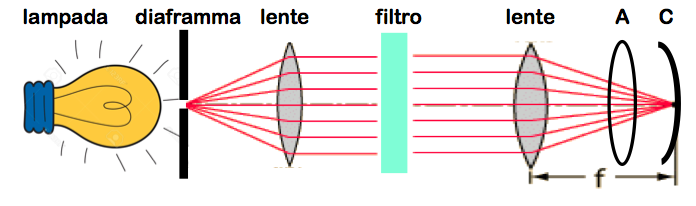
\includegraphics[scale=0.7]{lamp}
    \caption{Rappresentazione schematica dell'apparato di illuminazione della
    fotocella
    \label{fig: lamp}}
\end{figure}

Per variare la frequenza $\nu$ della radiazione che illumina la cella
fotoelettrica utilizziamo 4 filtri di tipo interferenziale, per cui la luce
trasmessa non è monocromatica, ma viene dispersa intorno al valore nominale
centrale secondo una distribuzione di intensità spettrale pressoché uniforme
su intervalli di larghezza $\text{FWHM} \approx 10 \; \si{n\m}$ attorno alla
lunghezza d'onda centrale CWL.

Teniamo conto della dispersione dello spettro incidente associando alla
lunghezza d'onda centrale (riportata nei rispettivi datasheet) un'incertezza
pari alla deviazione standard della curva di trasmissione a partire dalla
larghezza a metà altezza FWHM (anch'essa tabulata) secondo la formula
\[
\lambda \pm \sigma_\lambda = \text{CWL} \pm \text{FWHM}/\sqrt{12}
\]

Per variare la tensione $V\ped{bias} \in [0, 2] \; \si{\V}$, intervallo entro
il quale ci aspettiamo di trovare la tensione di frenamento critica $V_0$,
generiamo in \verb+WG1+ una rampa di tensione compresa tra i due estremi e la
misuriamo con il \verb+CH1+ dell'oscilloscopio di un AD2 secondo lo schema in
\cref{schm: Imeas}.
Con il secondo canale misuriamo contemporaneamente quella generata dal
convertitore corrente-tensione all'uscita del picoamperometro: nel
nostro setup il fattore di conversione vale $\kappa = \SI{1}{n\A/\V}$
($\pm 0.4 \%$ dato dall'incertezza sulla lettura della corrente)
per cui misuriamo $I = \kappa V_{CH2} = V \cdot 10^{-9} \; [\si{A}]$
\begin{figure}[htbp]
    \centering
	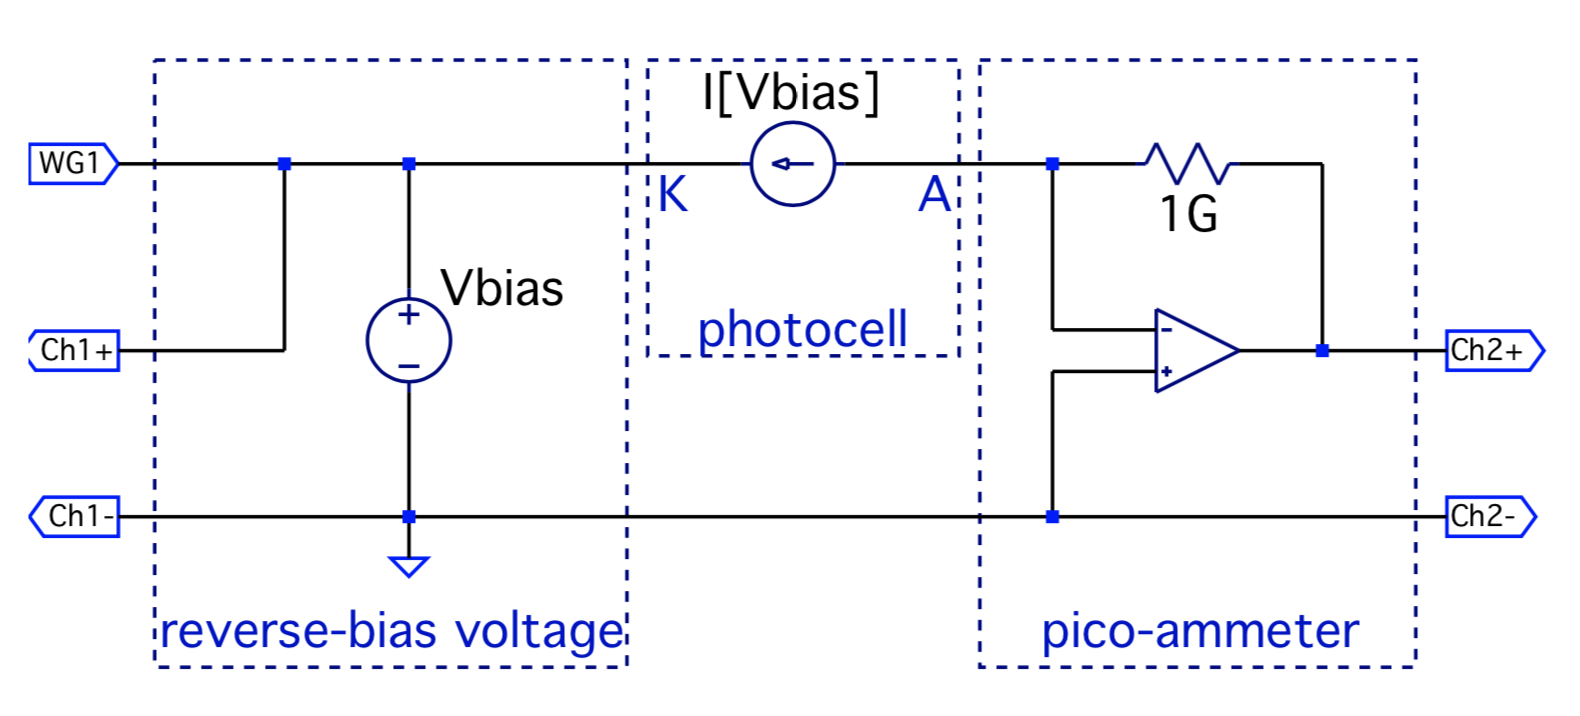
\includegraphics[scale=0.2]{schm}
    \caption{Schema del circuito equivalente per la misura dell'energia
    cinetica dei fotoelettroni.
    \label{schm: Imeas}}
\end{figure}

Finalmente usiamo la funzionalità di plot XY dell'oscilloscopio per ottenere
i grafici della corrente che attraversa la fotocella in funzione della
tensione di bias (come riportato a destra di \cref{fig: 546nm} in rosso le
ordinate Math1, sulle ascisse $V\ped{bias}$ misurata da CH1).

\subsection{Misura della corrente inversa}
Per effettuare la misura della corrente inversa abbiamo acquisito i dati come
sopra con la lampada accesa, con la sola differenza che il vano della
fotocella è stato opportunamente oscurato con un setto opaco, ricavando così
l'andamento della corrente inversa in funzione della tensione di bias nello
stesso intervallo di misura della fotocorrente riportato in \cref{fig: dark}
\begin{figure}[htbp]
    \centering
	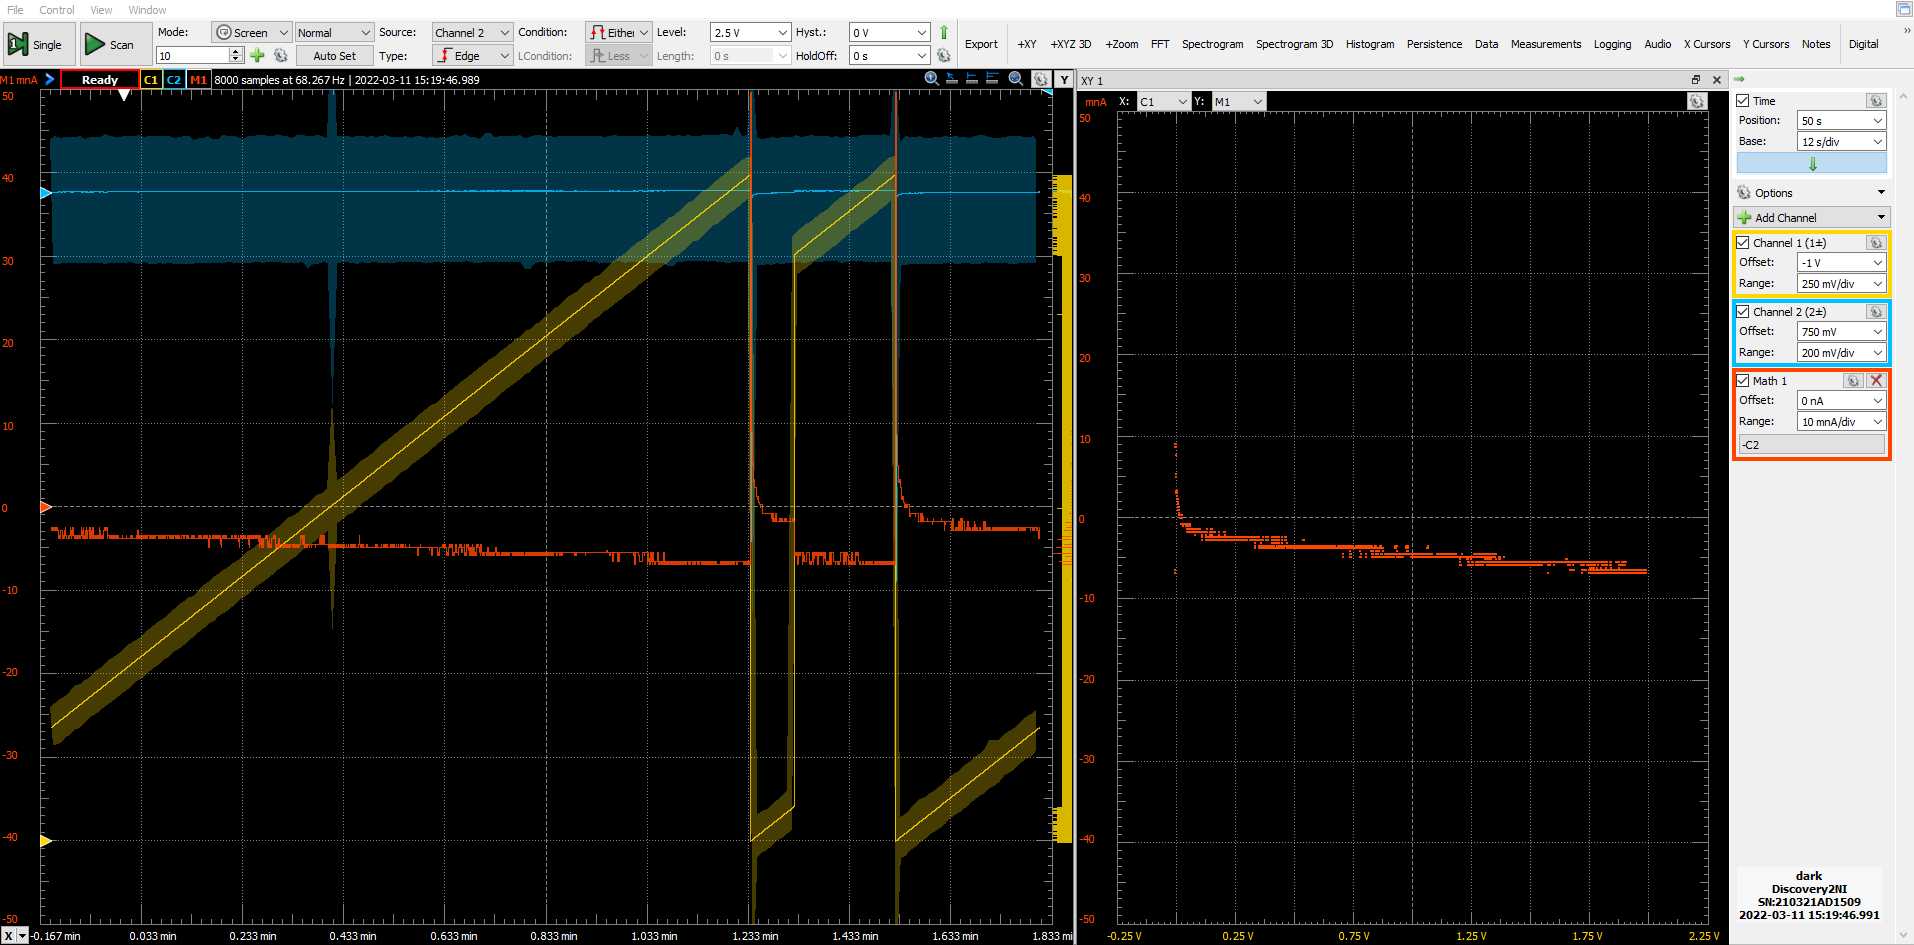
\includegraphics[width=\textwidth]{dark}
    \caption{Stampa a schermo dell'oscilloscopio per la misura della corrente
    senza luce incidente sulla cella fotoelettrica. Una volta superato il
    transiente iniziale all'inizio della rampa di tensione è già possibile
    notare un andamento lineare dei dati.
    \label{fig: dark}}
\end{figure}

%=======================
\section{Analisi dati e stima del rapporto $h/e$}
Abbiamo ottenuto una stima preliminare della tensione di azzeramento $V_0$
estraendo dalle curve corrente-tensione i valori di $V\ped{bias}$ per cui la
corrente anodica $I$ si discosta meno di due barre d'errore dalla corrente di
buio misurata senza luce incidente, da cui otteniamo:
\begin{table}
\centering
\begin{tabular}{cccccc}
\toprule
$\lambda \; [\si{n\m}]$ & $\sigma(\lambda) \; [\si{n\m}]$ &
$\nu \; [\si{T \Hz}]$ & $\sigma(\nu) \; [\si{T \Hz}]$ &
$V_0 \; [\si{\V}]$ & $\sigma(V_0) \; [\si{\V}]$ \\
\midrule
450 & 3 & 667 & 4 & 1.20 & 0.03 \\
499 & 3 & 601 & 4 & 0.99 & 0.03 \\
546 & 3 & 549 & 3 & 0.76 & 0.03 \\
577 & 3 & 520 & 3 & 0.64 & 0.03 \\
\bottomrule
\end{tabular}
\caption{Stime preliminari della tensione di frenamento critica $V_0$ trovate
al variare della frequenza della luce incidente sulla fotocella
\label{tab: V0prel}}
\end{table}

Dunque si è riusciti a stimare il valore del rapporto $h/e$ con un fit
lineare dell'andamento di $V_0$ in funzione di $\nu$, propagando
opportunamente gli errori sulle frequenze (in questo caso le incertezze sulla
variabile indipendente non sono trascurabili, in quanto
$\frac{h}{e} \sigma_\nu \sim \sigma_{V_0}$) che riportiamo in
\cref{fig: heprel}
\begin{figure}[htbp]
    \centering
	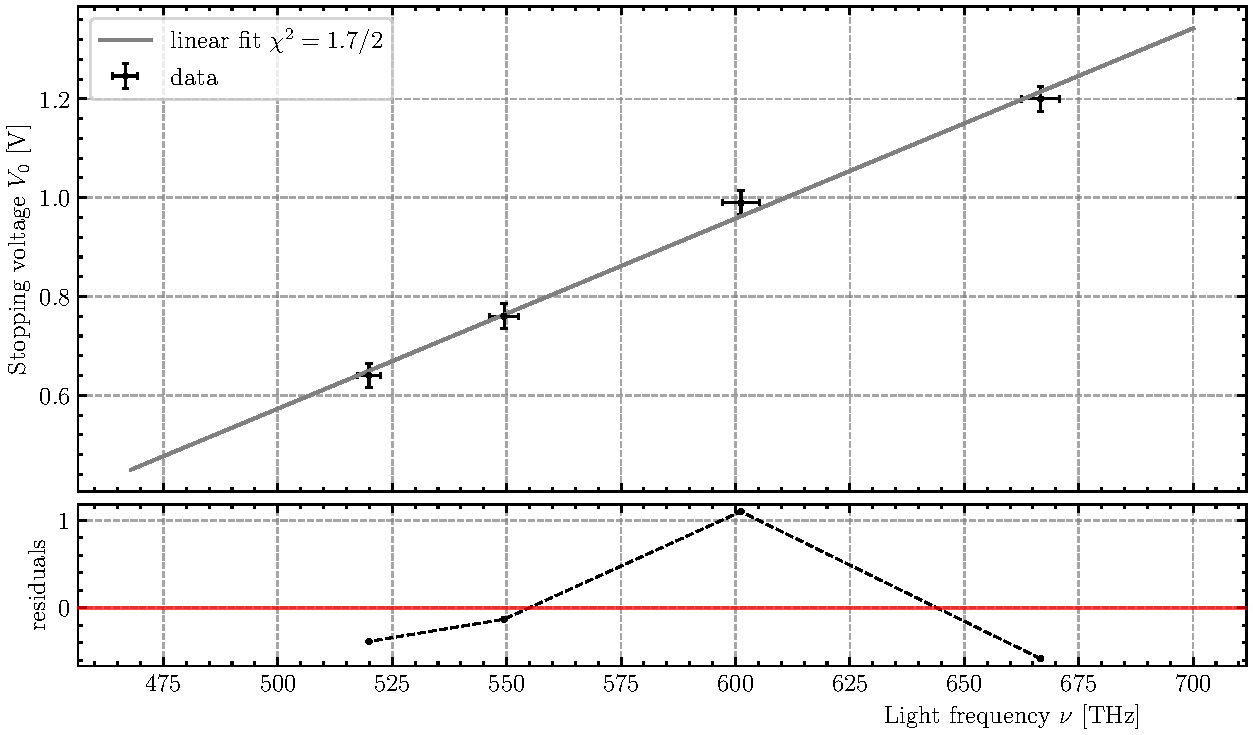
\includegraphics[width=\textwidth]{heprel}
    \caption{Grafico con retta di best-fit e residui normalizzati con i valori
    di $V_0(\nu)$ stimati in maniera grossolana dalle curve corrente-tensione.
    \label{fig: heprel}}
\end{figure}

\subsection{Metodo della corrente inversa}
Per studiare la corrente inversa eseguiamo un fit lineare sia sui dati
acquisiti per la corrente inversa senza luce incidente sia sui punti delle
curve della fotocorrente nella regione in cui $V\ped{bias} > V_0$ per ciascun
valore di lunghezza d'onda studiato.
Riportiamo i risultati dei fit in \cref{fig: darkfit} e \cref{tab: Invfit}
\begin{figure}[htbp]
    \centering
	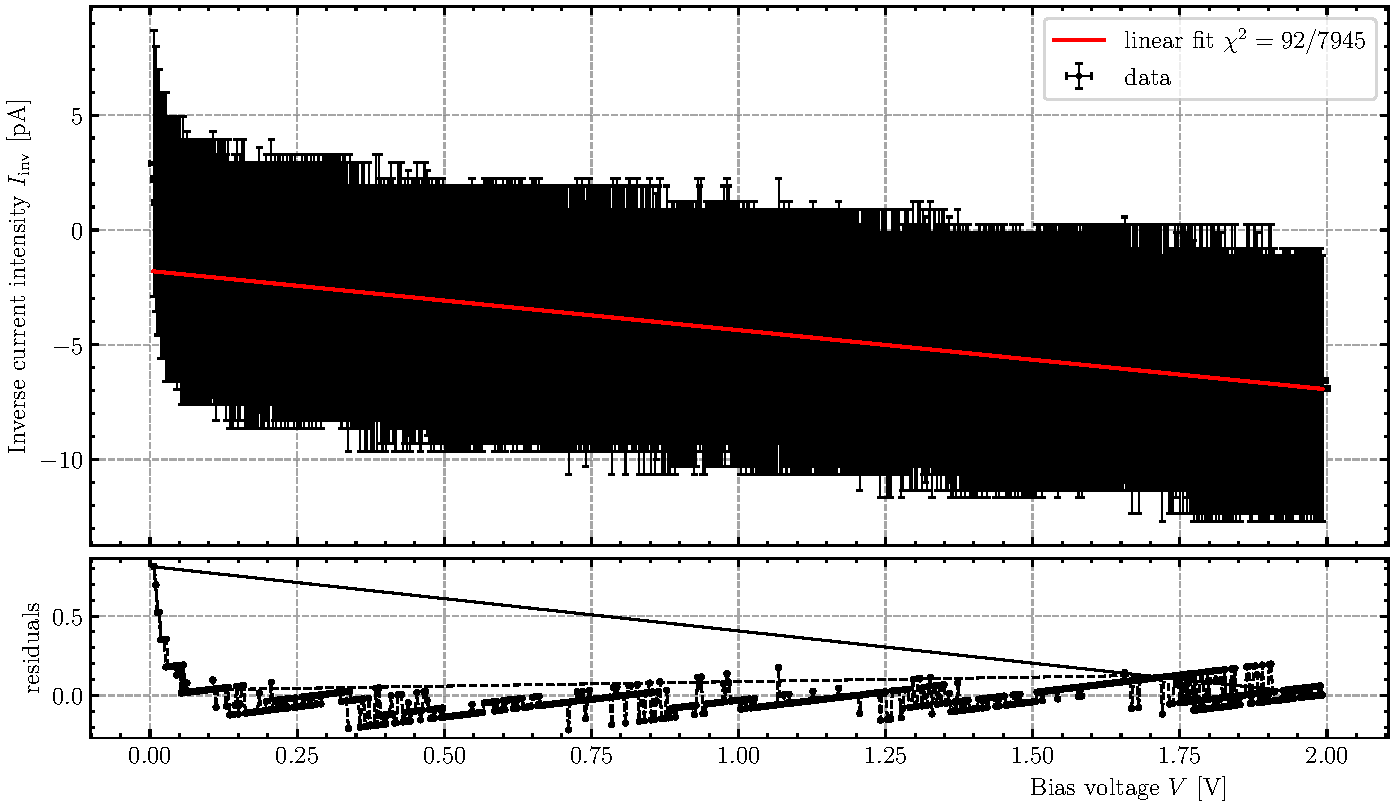
\includegraphics[width=\textwidth]{darkfit}
    \caption{Fit lineare all'andamento della corrente inversa $I\ped{inv}$ in
    funzione della rampa di potenziale di frenamento $V\ped{bias}$ in assenza
    di illuminazione
    \label{fig: darkfit}}
\end{figure}

\begin{table}
\centering
\begin{tabular}{ccccc}
\toprule
$\lambda \; [\si{n\m}]$ & $b \; [\si{p\mho}]$ & $I_0 \; [\si{pA}]$ &
$\chi^2/\text{ndof}$ & norm. cov. \\
\midrule
- &  $-2.58 \pm 0.10$ & $-1.78 \pm 0.13$ & $92/7945$ & $-0.858$ \\
$450 \pm 3$ & $-3.5 \pm 0.8$ & $-2.3 \pm 1.4$ & $8/2495$ & $-0.997$ \\
$499 \pm 3$ & $-1.9 \pm 1.0$ & $-4.6 \pm 1.7$ & $6/1689$ & $-0.997$ \\
$546 \pm 3$ & $-1.5 \pm 1.0$ & $-4.8 \pm 1.7$ & $11/1689$ & $-0.997$ \\
$577 \pm 3$ & $-1.7 \pm 1.0$ & $-4.5 \pm 1.7$ & $5/1688$ & $-0.997$ \\
\bottomrule
\end{tabular}
\caption{Risultati dei fit lineari per la misura della corrente inversa
al variare della lunghezza d'onda della radiazione incidente
\label{tab: Invfit}}
\end{table}

Da cui notiamo che, in primo luogo $I_0$ non risulta compatibile con $0$, né
indipendente dalla lunghezza d'onda della luce incidente, ma che nonostante
questo il modello lineare continua a descrivere fedelmente l'andamento dei
dati.

Anche per quanto riguarda il parametro $b$, i valori trovati dai 4 fit lineari
sulle fotocorrenti non risultano costanti al variare di $\lambda$, ma comunque
compatibili tra loro entro non più di due barre d'errore.

Prendendo una media pesata di questi si ottiene:
\begin{equation}\label{eq: bweight}
b = \frac{\sum_i b_i/\sigma_i^2}{\sum_i 1/\sigma_i^2} \pm
\frac{1}{\sqrt{\sum_i 1/\sigma_i^2}} = -2.1 \pm 0.5
\end{equation}
che risulta compatibile con il valore trovato dal fit sui dati senza luce
incidente.

Dunque possiamo ottenere dal fit lineare in assenza di illuminazione una stima
attendibile della resistenza equivalente percepita tra anodo e catodo
\[
1/\abs{b} = 388 \pm 16 \; \si{G\ohm}
\]
che risulta dello stesso ordine di grandezza atteso per via del cattivo
schermaggio tra gli elettrodi dovuto alle imperfezioni nelle guaine isolanti
dei cavi $(R \sim 10^{11-12} \; \si{\ohm})$.

Per provare a spiegare la dipendenza dei parametri del fit dalla frequenza
del fascio incidente notiamo che per le lunghezze d'onda più corte (per
fotoni più energetici) ci si aspetta che la tensione di azzeramento $V_0$ sia
più elevata, dunque che la corrente tenda più lentamente al suo valore
asintotico. Ipotizziamo che questo diverso andamento della corrente, dunque di
$I\ped{inv}$, al variare della lunghezza d'onda sia responsabile per la
dipendenza osservata dei parametri di fit da $\lambda$.

Da un primo fit con \cref{eq: Ifit} alle curve di fotocorrente acquisite,
lasciando tutti i parametri liberi si ottengono i risultati riassunti in
\cref{tab: Ifree} e \cref{fig: Ifree}
\begin{table}
\centering
\begin{tabular}{ccccccc}
\toprule
$\lambda \; [\si{n\m}]$ & $a \; [\si{p\A/\V^\alpha}] $ & $V_0 \; [\si{m\V}]$ &
$\alpha$ [arb. un.] & $b \; [\si{p\mho}]$ & $I_0 \; [\si{pA}]$ & $\chi^2/\text{ndof}$ \\
\midrule
$450 \pm 3$ & $492 \pm 3$ & $1273 \pm 2$ & $2.264 \pm 0.007$ & $-4.4 \pm 0.5$ &
$-0.6 \pm 0.8$ & $599/7817$ \\
$499 \pm 3$ & $756 \pm 4$ & $1061 \pm 2$ & $2.441 \pm 0.009$ & $-3.1 \pm 0.4$ &
$-2.5 \pm 0.6$ & $555/7817$ \\
$546 \pm 3$ & $1066 \pm 6$ & $863 \pm 3$ & $2.547 \pm 0.012$ & $-2.6 \pm 0.3$ &
$-2.9 \pm 0.4$ & $368/7817$ \\
$577 \pm 3$ & $1595 \pm 8$ & $751 \pm 3$ & $2.603 \pm 0.016$ & $-2.4 \pm 0.2$ &
$-3.2 \pm 0.3$ & $210/7817$ \\
\bottomrule
\end{tabular}
\caption{Risultati dei fit alle curve corrente-tensione con \cref{eq: Ifit}
lasciando tutti i parametri liberi.
\label{tab: Ifree}}
\end{table}

\begin{figure}[htbp]
    \centering
	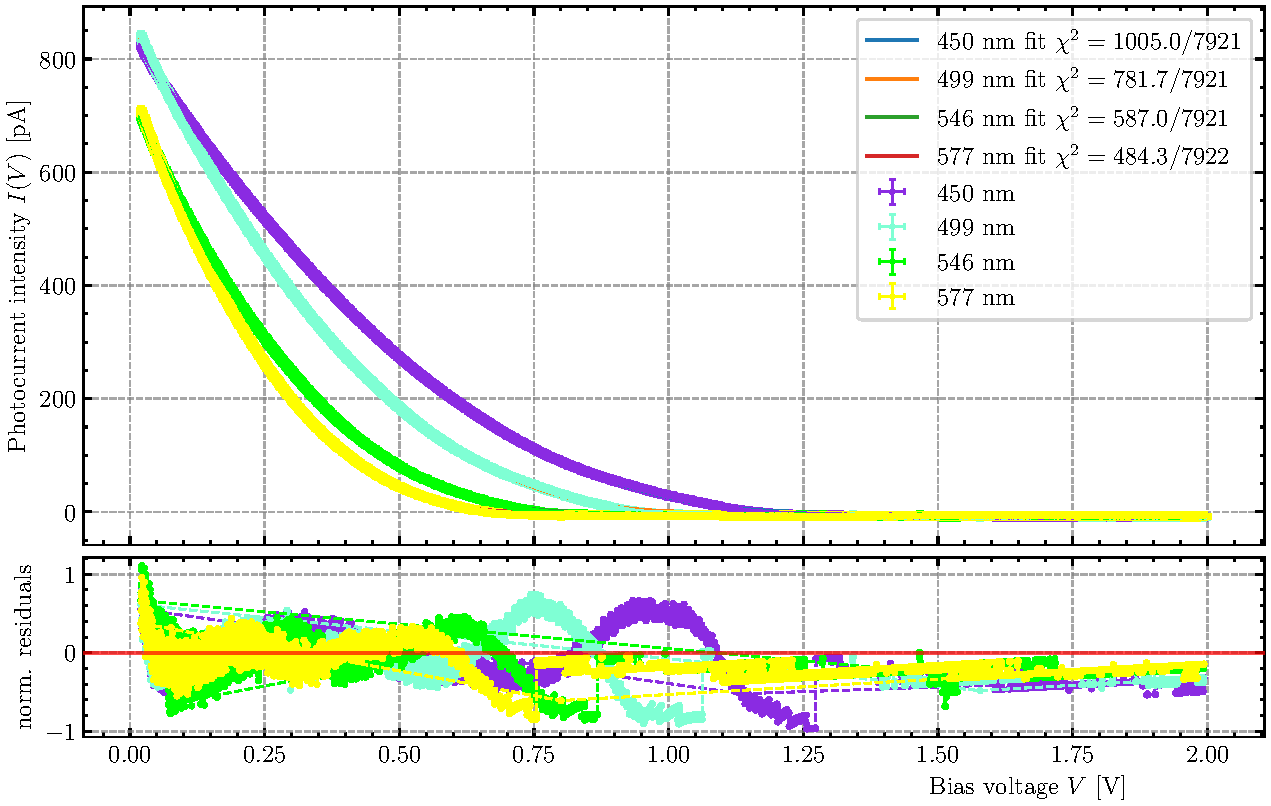
\includegraphics[width=\textwidth]{IV}
    \caption{Grafico dei fit con legge di potenza \cref{eq: Ifit} e residui
    normalizzati per le curve delle fotocorrenti acquisite in funzione del
    potenziale di frenamento $V\ped{bias}$
    \label{fig: Ifree}}
\end{figure}

Da cui possiamo osservare come tutti i parametri del fit assumono andamento
monotono in funzione della lunghezza d'onda, benché nel nostro modello
solamente i primi due dovrebbero racchiudere la dipendenza dalle
caratteristiche della luce incidente.
In particolare, i valori ottimali di $a$, $\alpha$ e $b$ risultano monotoni
crescenti in funzione di $\lambda$, mentre i parametri $V_0$ e $I_0$
(fortemente anticorrelati rispettivamente ad $a$ - $\alpha$ e $b$) hanno
andamento monotono decrescente.

Supponiamo quindi che gli $\alpha$ di best-fit risultino tutti sistematicamente
maggiori di $3/2$ e non compatibili tra di loro poiché nel nostro modello
consideriamo gli elettroni liberi nel metallo e non teniamo conto delle
successive interazioni dei fotoelettroni con il bulbo della fotocella.

\subsection{Dipendenza dei parametri ottimali dall'intervallo di misura}
Anche una volta fissati i valori di $I_0$ e $b$ dai risultati ottenuti nella
sezione precedente si è notato che la stima dei valori del potenziale frenante
critico $V_0$ e dell'esponente $\alpha$ continuavano ad esibire
un'apprezzabile dipendenza dall'intervallo di tensioni di bias considerate nei
fit della fotocorrente.

Considerando valori di $V\ped{bias} \sim 0$, oltre a quelle vicine al ginocchio
in $V_0$, si è visto che il valore dell'esponente $\alpha$ assume un
andamento monotono crescente in funzione della lunghezza d'onda in maniera
analoga a quello osservato per i parametri $a$ e $b$. Viceversa, restringendo
sempre di più i dati alla regione in cui $V\ped{bias} \sim V_0$, i valori
ottimali di $\alpha$ assumono valori tendenzialmente minori (di non più del
$20 \%$) di quelli in \cref{tab: Ifree}, ma con andamento difficilmente
prevedibile ed estremamente sensibile a variazioni dell'intervallo di misura.

Si è scelto quindi di fissare il valore di $\alpha$ come media pesata dei
valori ottimali stimati dai fit prendendo in considerazione l'intero range di
tensioni esplorato, dunque di eseguire un nuovo fit simultaneo ai 4 dataset
lasciando liberi solamente i restanti parametri dipendenti dalla frequenza
della luce incidente: $V_0$ e $a$.

Dal primo fit simultaneo con $\alpha$ parametro libero si trova, dalla
media pesata dei valori ottimali (come in \cref{eq: bweight})
\[
\alpha = 2.481 \pm 0.005
\]

dunque riportiamo i risultati del secondo fit simultaneo a due parametri, da
cui si sono ottenute le nostre misure più accurate della tensione di
azzeramento della fotocorrente $V_0$ in \cref{tab: inp} e \cref{fig: inp}
\begin{table}
\centering
\begin{tabular}{ccccc}
\toprule
$\nu \; [\si{T\Hz}]$ & $a \; [\si{p\A/\V^{2.481}}] $ & $V_0 \; [\si{m\V}]$ &
$\chi^2/\text{ndof}$ & norm. cov. \\
\midrule
$667 \pm 4$ & $411.9 \pm 0.6$ & $1345.6 \pm 0.6$ & $2070/7820$ & $-0.976$ \\
$601 \pm 4$ & $739 \pm 1$ & $1072.1 \pm 0.5$ & $806/7820$ & $-0.978$ \\
$549 \pm 3$ & $1097 \pm 2$ & $848.9 \pm 0.5$ & $522/7820$ & $-0.983$ \\
$520 \pm 3$ & $1644 \pm 4$ & $728.8 \pm 0.5$ & $505/7820$ & $-0.977$ \\
\bottomrule
\end{tabular}
\caption{Risultati dei fit con leggi di potenza con esponente $\alpha$ fissato
al variare della lunghezza d'onda $\lambda$ della radiazione incidente
\label{tab: inp}}
\end{table}

\begin{figure}[htbp]
    \centering
	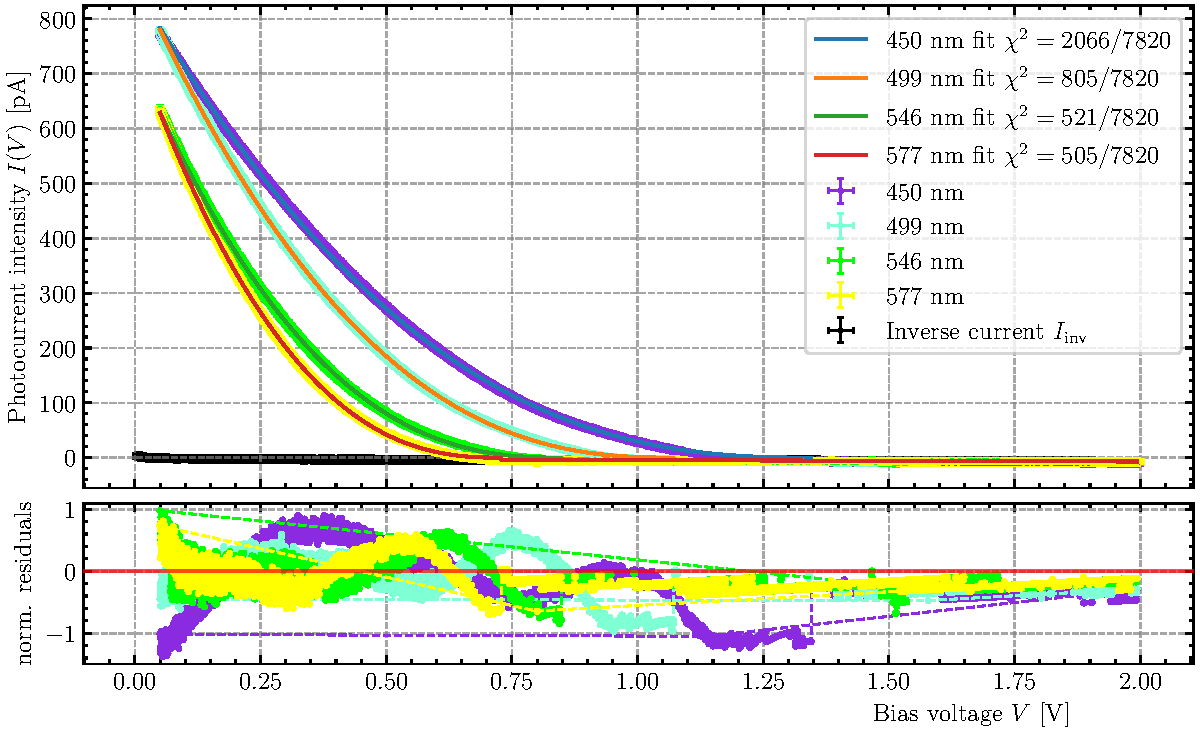
\includegraphics[width=\textwidth]{inp}
    \caption{Grafico del fit simultaneo con legge di potenza ($\alpha$ fissato)
    e residui normalizzati per le curve delle fotocorrenti acquisite in
    funzione della tensione $V\ped{bias}$
    \label{fig: inp}}
\end{figure}

Finalmente, dai valori di $V_0$ ricavati fissando l'esponente $\alpha$ al suo
valore ottimale proponiamo un fit lineare con la relazione inversa della
\cref{eq: V0}
\begin{equation}\label{eq: eh}
\nu = \frac{e}{h} V_0 - W_0/h
\end{equation}
dal momento che ora $\frac{h}{e} \sigma_\nu \gg \sigma_{V_0}$, per cui
possiamo trascurare le incertezze su $V_0$ nel fit ai minimi quadrati
(i cui risultati si riportano in \cref{fig: eh} e \cref{tab: he}).

\begin{figure}[htbp]
    \centering
	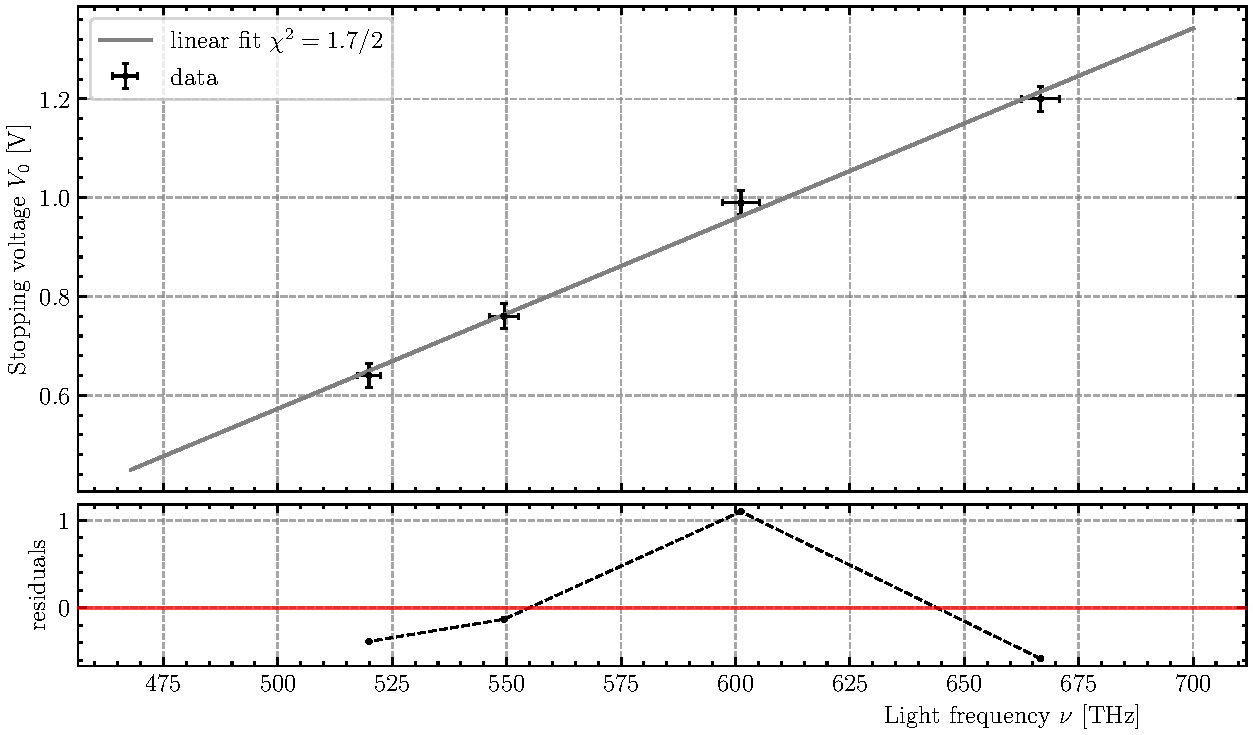
\includegraphics[width=\textwidth]{heprel}
    \caption{Grafico con retta di best-fit e residui normalizzati per la
    relazione inversa \cref{eq: eh}.
    \label{fig: eh}}
\end{figure}

\begin{table}
\centering
\begin{tabular}{ccccc}
\toprule
Metodo & $h/e \; [\si{\V \s}]$ & $W_0/e \; [\si{\V}]$ &
$\chi^2/\text{ndof}$ & norm. cov. \\
\midrule
Prel. & $3.9 \pm 0.2$ & $1.35 \pm 0.12$ & $1.7/2$ & $-0.995$ \\
$I\ped{inv}$ & $4.21 \pm 0.13$ & $1.46 \pm 0.21$ & $0.1/2$ & $-0.971$ \\
\bottomrule
\end{tabular}
\caption{Risultati dei fit lineari per la misura del rapporto $h/e$ ottenuti
dai due metodi impiegati: la stima preliminare e quello della corrente inversa
\label{tab: he}}
\end{table}

Da cui otteniamo come valore del rapporto $h/e = 4.21 \pm 0.13 \; \si{\V \s}$,
che è compatibile entro l'incertezza con il valore atteso.

%1/pars[0]
%Out[29]: 3.568317911720477
%Quindi un valore del rapporto h/e sottostimato di circa il $15 \%$ rispetto al
%valore atteso.

\subsection{Effetto fotoelettrico sull'anodo e lavoro di estrazione}
Dal datasheet della cella fotoelettrica sappiamo che questa è composta da un
anodo in lega di platino e rodio, che è una spira di $\SI{3}{c\meter}$ e da un
catodo in potassio rivestito di ossido d'argento, costituito da un arco
delle dimensioni di $\SI{4}{c\meter}$.

Per minimizzare il contributo alla corrente inversa dato dall'emissione di
fotoelettroni dall'anodo quando viene investito dagli aloni del fascio di
luce incidente si è ridotta l'apertura del diaframma così che la sua
immagine, messa a fuoco al centro del catodo, abbia dimensioni molto
inferiori al raggio dell'anodo.

Non solo: il potassio -come tipico per i metalli alcalini- ha lavoro di
estrazione $W\ped{0, K} \approx 2.15 \; \si{e\V}$ più basso di quello di altri
metalli, come il platino $W\ped{0, Pt} \approx 5.29 \; \si{e\V}$ con cui è
stato realizzato l'anodo sempre per questo motivo.

Dalla nostra analisi i risultati ottenuti per $W_0$ risultano compatibili con
il valore dell'intercetta attesa dal datasheet della fotocella e in
particolare risultano anche in accordo con il valore del lavoro di estrazione
del potassio. Prendendo nuovamente la media pesata dei valori ottimali come in
\cref{eq: bweight} infatti abbiamo
\[
W_0/e = 1.37 \pm 0.08 \; \si{\V} \implies W_0 = 2.19 \pm 0.12 \; \si{e\V}
\]

%=======================
\section*{Conclusioni e commenti finali}
Si è riusciti a dare una stima ragionevole del rapporto $h/e$ tramite due
varianti del metodo del potenziale frenante. Nonostante la semplicità della
procedura già da una stima preliminare si è riusciti ad ottenere un valore
con scarto dell'$8 \%$ circa. Con il metodo della corrente inversa si riesce
a migliorare significativamente la precisione (incertezza relativa del $3 \%$)
e l'accuratezza (scarto del $2 \%$) della misura dello stesso rapporto,
seppure questo richieda particolare attenzione nelle procedure di fit.

%=======================
\section*{Dichiarazione}
I firmatari di questa relazione dichiarano che il contenuto della relazione \`e
originale, con misure effettuate dai membri del gruppo, e che tutti i firmatari
hanno contribuito alla elaborazione della relazione stessa.

\end{document}
